\chapter{Introducción}\label{introduccion}

\section{Motivación y antecedentes}

A partir de los años 90 Internet tuvo una gran expansión, pasando de compartir información entre investigadores, 
como se hacía al principio, a permitir realizar compras, realizar videollamadas, pedir cita médicas, informes médicos, gestionar 
las cuentas bancarias, etc. Internet llega a millones de personas que consumen recursos de forma masiva. 
Existen múltiples aplicaciones que proporcionan el mismo servicio, por lo que es crucial tener cierta calidad de servicio 
\cite{microqos} para mantener una base de usuarios activos.

\intro Como se puede ver en la Figura \ref{Figura 1}, la calidad de servicio es fundamental para que el ancho de banda no se vea 
afectado por diferentes tipos de tráfico. Si se tienen, por ejemplo, tres tipos de tráfico distinto que ocupan el mismo ancho, al 
llegar al usuario final no se debe de permitir que uno ocupe todo el canal cortando los demás tipos de tráfico. Si se está realizando 
una videollamada, y esta ocupa todo el ancho de banda se tendrá como resultado que otros servicios no funcionen de forma correcta.

\intro Hay que tener en cuenta el tipo de aplicación que se está usando, para saber la prioridad que tiene. Por ejemplo, para 
enviar un correo da igual tener que esperar 1 minuto para que se envíe. Pero si se trata del visionado de una película por 
\textit{streaming} y hay retardo, no se cumplirá con los requisitos de calidad de servicio.

\intro Aparte de la calidad de servicio, también hay que tener en cuenta la seguridad, pues como ya se ha mencionado 
se tratan datos de tipo muy sensible, como son los datos bancarios y sanitarios. Este tipo de datos están protegidos por la Agencia 
Española de Protección de Datos \cite{aepdindex} y la Ley Orgánica de Protección de Datos \cite{lopdindex}.

\begin{figure}[H]
  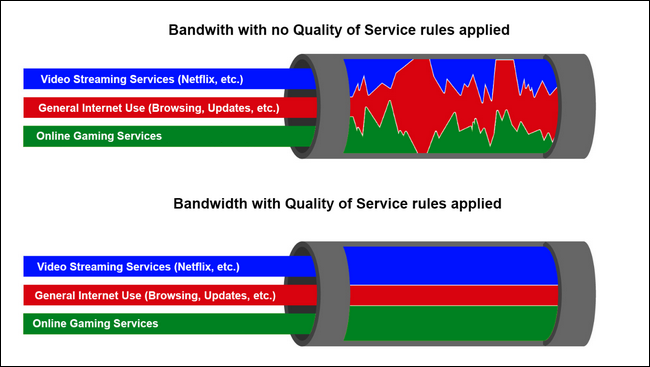
\includegraphics[width=0.75\textwidth]{imagenes/calidadservicio.png}
  \centering
  \caption{Ejemplo del ancho de banda sin calidad de servicio y con calidad de servicio.}\label{Figura 1}
\end{figure}

\intro Se puede dar prioridad a diferentes tipos de tráfico mediante su identificación y posterior clasificación. ``La identificación 
del tráfico consiste en atribuir instancias o elementos de tráfico a las aplicaciones que lo generaron" \cite{jawad2016}. Esto puede 
ser realizado siguiendo tres niveles. A nivel de flujo, a nivel de paquete y a nivel de equipos. Siendo el más común la clasificación 
a nivel de flujo.

%\intro Existe una forma de dar prioridad a diferentes tipos de tráfico, mediante la identificación de este y su posterior clasificación. La identificación de tráfico consiste en analizar el tráfico de una red y mediante alguna de las distintas técnicas existentes organizarlo mediante patrones comunes, como por ejemplo podría ser las IP's y los puertos, el contenido de las cabeceras de los paquetes o mediante técnicas heurísticas. Mediante estas técnicas se podrá dar prioridad a un tipo de tráfico sobre otro, mejorando así la calidad de servicio.

\intro Dentro de las técnicas de identificación de tráfico, la más fiable es la Inspección Profunda de Paquetes, DPI o \textit{Deep Packet Inspection} en inglés\cite{dpiaproximacion}. Consiste en analizar los paquetes más allá de la cabecera, buscando cadenas que 
permitan identificar inequívocamente el protocolo. Por ejemplo buscará para \textit{HTTP} las cadenas \textit{GET} y \textit{POST}.

\intro Esta técnica, a pesar de ser la más efectiva cuenta con varios inconvenientes.
\begin{itemize}
\item \textit{Escalabilidad}. Ya que se trata de una técnica que tiene que ir paquete a paquete y entrar dentro de ellos requiere de 
una gran cantidad de recursos. Si se trata de analizar una red con poco tráfico, se obtendrán buenos resultados en cuanto a 
rendimiento, pero de tratarse de una red con mucho tráfico, se tendrán malos tiempos de análisis.
\item \textit{Privacidad}. Al entrar dentro de los paquetes, se produce cierta violación de las políticas de privacidad de la red. Si 
se trata de una red local no hay problemas. Pero si se trata de una red pública si que se incurre en violaciones de privacidad.
\end{itemize}

\intro Una solución parcial a este problema podría ser la aplicación de la técnica de emparejamiento de flujos \cite{presentacion}, 
desarrollada por el departamento de Teoría de la Señal, Telemática y Comunicaciones, TSTC, de la Universidad de Granada y probada en 
entornos de laboratorio \cite{comparacion}. Esta técnica además de ser eficiente, respeta la privacidad al no inspeccionar de forma 
profunda los paquetes.

\intro Por lo tanto, en el presente trabajo se va a implementar esta técnica y se probará más allá de un entorno de laboratorio, 
llevándola a escenarios reales.

\intro Para llevar esta técnica a un escenario real se precisará de un monitor de redes, NMS, \textit{Network Monitoring System}. 
El trabajo que realiza es el de monitorizar el tráfico en la red en la que se esté ejecutando.
Para este proyecto se usará Bro \cite{broindex}, cuya principal ventaja sobre el resto es la posibilidad de incorporar funcionalidades 
extras. Esto se realiza mediante la creación de módulos.

\section{Objetivos}

El objetivo de este trabajo es el desarrollo de un módulo para un NMS, en este caso Bro. Con el desarrollo del módulo se tratará 
de demostrar que la técnica de emparejamiento de flujos se puede realizar fuera de un entorno de laboratorio.

\intro Este objetivo se descompone de la siguiente forma.

\begin{itemize}
\item Gestión de las entradas y salidas. En un principio se hará uso de un archivo \textit{pcap}, de forma 
que se pueda comprobar que todo funciona correctamente. Una vez terminado será posible realizar una ejecución a tiempo real en una 
red.
\item Implementación de la función de emparejamiento de flujos, así como el control de los distintos eventos para la gestión del 
tráfico.
\item Realización de pruebas del funcionamiento.
\end{itemize}

\section{Metodología}

Para realizar este trabajo se establecen una serie de tareas:

\begin{itemize}
\item Estado del Arte.
	\begin{itemize}
	\item Lectura del artículo del departamento. \cite{comparacion}
	\item Búsqueda de información sobre la identificación de tráfico.
	\item Análisis de las herramientas.
	\end{itemize}
\item Diseñar el módulo.
\item Implementar el módulo.
\item Evaluación y pruebas del módulo.
\item Realización de la memoria.
\end{itemize}

\intro En la siguiente Figura \ref{fig.tempo}, se puede ver una temporización de las tareas en forma de diagrama de Gantt.

\begin{figure}[H]
  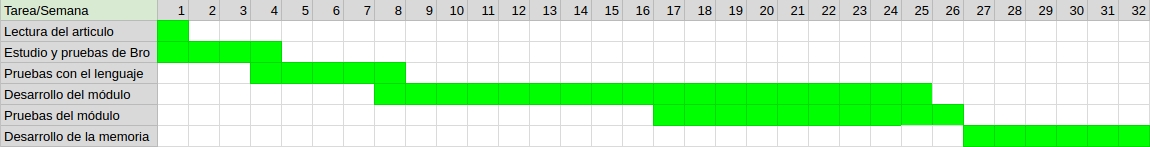
\includegraphics[width=1\textwidth]{imagenes/temporizacion.png} 
  \centering
  \caption{Temporización en diagrama de Gantt.}\label{fig.tempo}
\end{figure}

El gasto que requiere este proyecto se desglosa de la siguiente manera.
\begin{itemize}
\item \textit{Licencias}. El gasto en licencias será nulo, pues Bro está creado bajo licencia de software libre \cite{broindex}. El 
módulo será subido a GitHub \cite{repo} con licencia de software libre, por lo que cualquiera podrá usarlo o modificarlo en el futuro.
\item \textit{Equipo}. Teniendo en cuenta que la vida útil de un portátil es de unos 4 años y que el desarrollo de este trabajo 
requiere de unos 6 meses, se tendrá que un portátil de gama media-alta de 800\euro generará un gasto de un octavo de la vida útil. Por 
lo tanto será un coste de unos \textit{100\euro}. Hay que tener en cuenta que Bro solo funciona en Linux o Mac OS X 
\cite{brodownload}.
\item \textit{Programador}. Según se puede comprobar en Internet \cite{tarifa}, el precio por hora de un programador está alrededor de  
los 30\euro, por lo tanto si en el desarrollo del proyecto se ha necesitado de unas 500 horas y dejando el precio en 30\euro por hora, 
el gasto será de \textit{15000\euro}.
\item \textit{Varios}. Además de los gastos ya descritos, hay que sumar una parte de gastos varios como Internet, luz, agua, y 
demás. Un montante de 150\euro al mes, que al ser 6 meses supone un gasto de \textit{900\euro}.
\end{itemize}

\intro Teniendo en cuenta todos estos cálculos, se tiene que el coste total del proyecto es de unos \textit{16000\euro} por 6 meses de 
trabajo.

\section{Estructura de la memoria}

Esta memoria se organizará de la siguiente forma: 
\begin{itemize}
\item En el capítulo \ref{estadoarte} se hablará de todos los fundamentos teóricos y tecnológicos sobre los que se 
basa el proyecto.
\item En el capítulo \ref{diseno} se contará cómo se pretende resolver el problema expuesto.
\item En el capítulo \ref{implementacion} se encontrará detallado cómo se han implementado los diferentes módulos.
\item En el capítulo \ref{evaluacion} se realizarán las pruebas, para comprobar que todo funciona como 
estaba previsto, tanto a nivel funcional como a nivel de aplicación.
\item En el capítulo \ref{conclusiones} se hablará de las conclusiones recogidas a lo largo de este proyecto y las posibles 
opciones que tiene para seguir trabajando sobre él.
\end{itemize}
